\documentclass[11pt,oneside]{scrbook}
\usepackage[a4paper,left=2.4cm,right=4.2cm,top=2.4cm,bottom=2.4cm,marginparwidth=2.6cm,marginparsep=0.5cm]{geometry}
\usepackage{../common/rlstudy}
\usepackage[ruled,vlined]{algorithm2e}
\usepackage{longtable}
\title{\color{rlblue}\textbf{Week 26: Causal discovery across biological environments}\\\large Noisy patient observations, task-aware enhancement, and the limits of prediction}
\author{STUDY-RL}
\date{Research checked October 5, 2026}

\begin{document}
\maketitle
\tableofcontents

\chapter*{Learning objectives}
\addcontentsline{toc}{chapter}{Learning objectives}
\begin{keyidea}
By the end of this week, you should be able to:
\begin{enumerate}
\item distinguish a prediction, an intervention effect, and a discovered graph;
\item derive standardization from consistency, exchangeability, and positivity;
\item construct observationally equivalent SCMs with different intervention responses;
\item explain how changing environments may help identification, and when they do not;
\item distinguish PC, FCI, S-FCI, and ICP from the project's descriptive diagnostics;
\item prevent patient and preprocessing leakage in a noisy-data experiment;
\item compare enhancement with an unchanged baseline and an informative ablation.
\end{enumerate}
\end{keyidea}
Use \texttt{teaching\_guide.md} as the entry point, then execute
\texttt{workbook.ipynb}. The five-session study plan requires approximately ten hours.
The code runs on CPU using NumPy. All outcomes in the project are synthetic.

\chapter{Motivation \& intuition}
\section{What question are we asking?}
Imagine a marker strongly associated with a disease phenotype. A predictive model can
use that association without knowing why it exists. The marker could be a cause, a
consequence, a proxy for another process, or an artifact of sample selection.
The intervention question is different: what would change if we altered the marker's
generating mechanism? The answer depends on a causal model, a well-defined intervention,
and the population in which the intervention is considered.

This week was prompted by Synlico's discussion on learning from patient data across
environments and enhancing noisy, sparse biological measurements. The public event listing
is contextual motivation, not an experimental result. The company describes a proprietary
enhancement system; its unpublished implementation is not reproduced here.
\marginnote{Event topic, peer-reviewed method, and company performance claim have different provenance.}

\begin{center}
\begin{tabular}{p{0.24\textwidth}p{0.65\textwidth}}
\toprule
Question & What must be specified?\\
\midrule
Prediction & Measured inputs, outcome, loss, and evaluation distribution.\\
Effect estimation & Intervention, potential outcomes, target population, and identification assumptions.\\
Discovery & Graph family, observed variables, hidden-variable assumptions, and identifying evidence.\\
Target validation & Perturbation, controls, timing, relevant cell state, and biological response.\\
\bottomrule
\end{tabular}
\end{center}

A useful drug-discovery workflow can move from a computational hypothesis to a controlled
perturbation and then further validation. Each stage supplies a different kind of evidence.
A hypothesis is not invalid because it remains uncertain, but its uncertainty should
remain visible. Neither a low reconstruction error nor a confident arrow proves that a
drug intervention will benefit patients.

\section{Analogy: kitchens and recipe mechanisms}
Different kitchens prepare the same dish. Oven temperature affects doneness, while a
camera records its appearance. One kitchen changes the temperature distribution;
another changes its lighting. Temperature maps to a candidate cause $X$, doneness
to a target $Y$, and lighting to a measurement or proxy mechanism. Ingredient quality
$C$ could affect both temperature choice and doneness. Unrecorded humidity could be a
latent common cause.

The equation $Y=f_Y(X,C,U_Y)$ is the recipe mechanism. A setting
\(\operatorname{do}(X=x)\) replaces the oven-setting rule rather than selecting dishes
that happened to be cooked at temperature $x$. An environment $E=e$ labels a kitchen
whose distributions or mechanisms may differ.

\begin{pitfall}
The recipe itself can change. Tissue, cell state, time, disease, or selection can alter
the target mechanism. The kitchen analogy motivates a conditional-invariance question;
it does not prove invariance or safe intervention in biology.
\end{pitfall}

\section{Biological environments are not interchangeable batches}
An environment can be a study, patient group, tissue, experimental condition, or measurement
protocol. These labels describe different possible changes. A tissue change can alter
regulation and cell composition. A sequencing change can alter the observation mechanism.
A study can select a different patient population. Pooling such observations without the
labels can conceal information, whereas removing every environment difference can also
remove biologically informative variation.

The modeler must explain which variables correspond across environments and which
mechanisms are permitted to change. A batch label is not a randomized intervention.
Strong cross-environment identification statements require the assumptions of the particular
method being used.

\section{The unit of evidence}
Ten thousand cells from ten patients do not automatically provide ten thousand independent
patients for estimating a patient-level effect. Cells may share donor biology, sample
preparation, treatment, and outcome. A model can recognize donor information and appear
to generalize when one donor's cells occur in both training and testing.

Our project therefore uses repeated technical measurements and globally unique patient
IDs. Every repeated row stays with its patient. The simplified target is shared across
the patient's measurements, making row leakage easy to recognize. This fixture is not a
mechanistic cell population model.

\section{Relation to previous weeks}
Week 11's support problem reappears as treatment positivity. Week 12 separates exposure
from relevance, reminding us that measurements arise through a mechanism. Week 14 warns
about unsupported action extrapolation. Week 25 connects evaluation claims to their
evidence. Here we add graph identification and mechanism changes. No RL optimizer can
repair a missing causal assumption simply by optimizing longer.

\chapter{Mathematical formulation}
\section{Variables and a structural causal model}
\begin{definition}[Directed acyclic graph]
A DAG $G=(V,\mathcal E)$ has directed edges and no directed cycle. The parents
$\operatorname{pa}_G(V_j)$ are variables with arrows into $V_j$. An arrow encodes
a proposed direct structural dependence at the modeled resolution, rather than a large
sample correlation.
\end{definition}

\begin{definition}[Structural causal model]
An SCM supplies assignments $V_j=f_j(\operatorname{pa}_G(V_j),U_j)$ and a joint
distribution of disturbances $U=(U_1,\ldots,U_d)$. Independent disturbances represent
causal sufficiency in the simple acyclic setting; dependent disturbances can encode
latent common causes. The graph, assignments, and disturbance distribution together
specify intervention predictions.
\end{definition}

For effect estimation, use patient-level variables: binary treatment $A$, pre-treatment
covariate $C$, and later outcome $Y$. For prediction, use true markers $Z,C$, measured
versions, proxy $S$, and environment $E$. These are separate experiments in the code;
the prediction experiment does not define a treatment policy.

\begin{figure}[ht]
\centering
\begin{tikzpicture}[node distance=2.0cm,>=Stealth,every node/.style={draw,circle,minimum size=9mm}]
\node (c) {$C$};
\node[below left=of c] (a) {$A$};
\node[below right=of c] (y) {$Y$};
\draw[->,thick] (c)--(a);
\draw[->,thick] (c)--(y);
\draw[->,thick] (a)--(y);
\node[right=2.0cm of y,dashed] (u) {$U$};
\draw[->,dashed] (u) to[bend right=22] (a);
\draw[->,dashed] (u)--(y);
\end{tikzpicture}
\caption{Solid arrows show a measured-confounder model. If the dashed hidden
common cause is also present, adjusting for $C$ alone generally does not identify the effect.}
\end{figure}

\section{Observation versus intervention}
Conditioning on $A=a$ selects units whose original assignment rule produced $a$.
An intervention $\operatorname{do}(A=a)$ replaces that rule with the constant $a$.
The outcome and covariate assignments remain as specified by the intervention model.

For example, consider $C=U_C$, $A=f_A(C,U_A)$, and
$Y=\tau A+\gamma C+U_Y$. Conditioning can change the distribution of $C$ because
$A$ depends on $C$. Intervention does not condition on the old treatment assignment.
If $\E[U_Y]=0$ and the intervention leaves the distribution of $C$ unchanged,
\[
\E[Y\mid\operatorname{do}(A=a)]=\tau a+\gamma\E[C].
\]
The difference for $a=1$ and $a=0$ is $\tau$. By contrast, the observed difference is
\[
\E[Y\mid A=1]-\E[Y\mid A=0]
=\tau+\gamma\{\E[C\mid A=1]-\E[C\mid A=0]\}
\]
if $U_Y$ has zero conditional mean in both groups. The second term is the composition
effect in this simple model. With hidden common causes, another term can appear.

\section{Potential outcomes and the target population}
\begin{definition}[Average treatment effect]
For a specified target population, $Y(a)$ is the outcome under treatment version $a$.
The average treatment effect is
$\tau_{\mathrm{ATE}}=\E[Y(1)-Y(0)]$.
The expectation includes the population's distribution of baseline variables.
\end{definition}

An intervention must have a meaning beyond a binary column. Dose, duration, timing,
co-interventions, follow-up, and outcome measurement can distinguish treatment versions.
The simple binary fixture omits those complications. A molecular knockout response is
also a different estimand from a patient's response to a medication.

\begin{theorem}[Standardization under measured-confounder assumptions]
Assume $C$ is categorical and measured before treatment. For $a\in\{0,1\}$, assume:
\begin{enumerate}
\item consistency: $Y=Y(a)$ on units receiving the relevant treatment version $a$;
\item conditional exchangeability: $Y(a)\indep A\mid C$;
\item positivity: $P(A=a\mid C=c)>0$ for every target stratum with $P(C=c)>0$.
\end{enumerate}
Assume the observations concern this target population and that the expectations exist.
Then
\[
\tau_{\mathrm{ATE}}=\sum_c P(C=c)
\{\E[Y\mid A=1,C=c]-\E[Y\mid A=0,C=c]\}.
\]
\end{theorem}

\begin{proof}
Fix $a$. Apply the law of total expectation:
\[
\E[Y(a)]=\sum_c \E[Y(a)\mid C=c]P(C=c).
\]
Conditional exchangeability permits adding treatment conditioning without changing
each stratum's potential-outcome expectation:
\[
\E[Y(a)\mid C=c]=\E[Y(a)\mid A=a,C=c].
\]
Consistency replaces the potential outcome by the observed outcome among those
who actually received that version:
\[
\E[Y(a)\mid A=a,C=c]=\E[Y\mid A=a,C=c].
\]
Positivity ensures that these observed conditional expectations exist for target strata.
Substitute the last two equalities into the first expression. Do this once for $a=1$
and once for $a=0$. Subtract the two expressions and distribute the common target
weight $P(C=c)$ inside the sum. This gives the stated formula.
\end{proof}

This is an identification result about population distributions. Estimation replaces
unknown quantities by data summaries. The assumptions are not proven by a large sample
or a small regression loss. Hern\'an and Robins' \emph{What If} provides the foundational
framework; the derivation above is supplied explicitly for this course.

\section{A fully calculated reversal}
The following counts and scores are teaching fixtures, not medical evidence. There
are 100 mild and 100 severe patients. In the mild stratum, 20 treated have mean 3 and
80 untreated have mean 2. In the severe stratum, 80 treated have mean 1 and 20 untreated
have mean 0. Each within-stratum treatment difference is one.

Before computing, predict whether the pooled comparison will preserve the sign.
The treated total score is $20(3)+80(1)=140$, across 100 treated patients.
Its mean is $1.4$. The untreated total is $80(2)+20(0)=160$, across 100 untreated
patients, giving $1.6$. The pooled difference is $-0.2$.

The target proportions are $0.5$ and $0.5$, so standardization gives
\[
0.5(3-2)+0.5(1-0)=1.
\]
Using the same target mixture for each treatment arm removes the measured composition
difference. A target with proportions $(0.8,0.2)$ still has effect one because the
two stratum effects are identical. If the effects differed, transport to another
population would change the weighted ATE even if both conditional effects were stable.

If the severe untreated cell is empty, its mean is unavailable. An outcome model could
extrapolate, but that would introduce an additional assumption. The reference solution
raises \texttt{ValueError} instead of producing a support-free number.

\section{Paths, mediators, and colliders}
The path $A\leftarrow C\rightarrow Y$ is a backdoor path because it starts with an
arrow into treatment. In the simple measured-confounder DAG, conditioning on $C$
blocks it. More generally, a valid adjustment set requires graphical and substantive
reasoning. It is not the set of every recorded variable.

A mediator on $A\rightarrow M\rightarrow Y$ carries part of the treatment effect.
Conditioning on it can remove part of a total effect or introduce other bias. A collider
$X\rightarrow K\leftarrow Z$ has two incoming arrows; conditioning on $K$ can make
otherwise independent causes dependent.

Here is a calculated collider example. Let $X,Z$ be independent standard normals and
$K=X+Z$. Define $D=(X-Z)/\sqrt{2}$ and $B=(X+Z)/\sqrt{2}$. They are jointly Gaussian,
each has variance one, and
\[
\Cov(B,D)=\tfrac12\E[(X+Z)(X-Z)]=\tfrac12(1-1)=0.
\]
Thus $B,D$ are independent. Conditioning on $K$ fixes $B=K/\sqrt2$, while $D$
remains standard normal. Because $X=(B+D)/\sqrt2$ and $Z=(B-D)/\sqrt2$,
\[
\Cov(X,Z\mid K)=\Cov(D/\sqrt2,-D/\sqrt2)=-\tfrac12.
\]
Both conditional variances are $1/2$, giving conditional correlation $-1$.
Selection can therefore manufacture a strong relationship even before enhancement.

\section{Observational equivalence: a full counterexample}
\begin{proposition}[Two directions with one observational distribution]
Let $U,V$ be independent standard normal disturbances and $0<|\rho|<1$.
Consider
\[
\text{F: }X=U,\quad Y=\rho X+\sqrt{1-\rho^2}V
\]
and
\[
\text{R: }Y=U,\quad X=\rho Y+\sqrt{1-\rho^2}V.
\]
Their observational distributions agree, but their mean response of $Y$ to
$\operatorname{do}(X=x)$ differs when $\rho x\ne0$.
\end{proposition}
\begin{proof}
Both means are zero. In F, $\Var(X)=1$ and, using independent disturbances,
\[
\Var(Y)=\rho^2\Var(U)+(1-\rho^2)\Var(V)=1,
\quad \Cov(X,Y)=\rho\Var(U)=\rho.
\]
The same calculation with $X,Y$ exchanged gives the covariance matrix
\(
\begin{pmatrix}1&\rho\\\rho&1\end{pmatrix}
\)
in R. Both vectors are jointly Gaussian, so equal mean vectors and covariance
matrices imply identical joint distributions. In F, replacing $X=U$ with $X=x$
gives $Y=\rho x+\sqrt{1-\rho^2}V$, whose mean is $\rho x$.
In R, replacing the assignment for $X$ leaves $Y=U$ unchanged, with mean zero.
Thus observational agreement does not imply interventional agreement.
\end{proof}

At $\rho=0.8$, $\sqrt{1-\rho^2}=0.6$. The variance calculation is
$0.64+0.36=1$, while intervention means at $x=1$ are $0.8$ and $0$.
This is an identification obstruction: an unlimited observational sample does not
choose between these two models without additional assumptions or evidence.
Hidden-confounder models can add further explanations.

\section{Markov assumptions and what remains unoriented}
In the basic causally sufficient DAG model, the Markov property relates graph separation
to conditional independence, and faithfulness rules out some parameter cancellations
that would create additional independences. Two DAGs can encode the same independence
relations. A CPDAG summarizes that equivalence class with compelled and unresolved edges.
When latent causes are permitted, a PAG uses endpoint marks to summarize the causal
information retained across compatible ancestral graphs. A circle endpoint is unresolved;
it is not a confident causal direction.

The scope of these summaries depends on the model assumptions and quality of conditional
independence tests. Finite samples, repeated cells, measurement noise, and selection can
make the observed independences misleading. Biological feedback can also challenge an
acyclic representation. One can model time-indexed variables or use a framework for
cycles, but one should not silently apply an acyclic theorem to a feedback system.

\section{Conditional invariance across environments}
\begin{definition}[Target-mechanism invariance]
For environments $e$, a predictor set $S$ has conditional invariance for target $Y$
if the conditional law $P^e(Y\mid X_S=x)$ is the same over the relevant common support.
This is stronger than equality of marginal means or prediction errors.
\end{definition}

In a simple SCM, suppose
\(Y=\beta^\top X_S+U_Y\), the coefficient $\beta$ and disturbance distribution
are unchanged, and $U_Y$ is independent of $X_S$ in each environment. Then conditioning
on $X_S=x$ leaves the same distribution $\beta^\top x+U_Y$ in every environment.
Different marginal distributions of $X_S$ need not change that conditional law.
The conclusion follows directly from the assignment and independence assumptions.

It can fail if an environment changes the target equation, alters unobserved causes,
selects observations, or changes measurement. Invariance may also hold for multiple
predictor sets, so stability alone need not identify every parent. ICP uses a formal
testing construction; the project's residual spread does not implement that construction.

\begin{figure}[ht]
\centering
\begin{tikzpicture}
\begin{axis}[width=0.91\textwidth,height=5.1cm,xlabel={True marker $Z$},ylabel={Conditional mean target},legend pos=north west,grid=major]
\addplot[rlblue,thick,domain=-2:2] {1.5*x};
\addlegendentry{Stable target mechanism}
\addplot[rlorange,dashed,thick,domain=-2:2] {2.5*x};
\addlegendentry{Changed target mechanism}
\end{axis}
\end{tikzpicture}
\caption{A predictor-parent mechanism can remain stable under covariate changes,
but a change in the target equation defeats this invariance premise. The lines are teaching equations.}
\end{figure}

\section{Noise, missingness, and manufactured dependencies}
Write a measured marker as $W=X+\epsilon$, with independent mean-zero measurement
error. If $Y=\beta X+U$ and all disturbances are mutually independent, the population
least-squares coefficient of $Y$ on $W$ is
\[
\frac{\Cov(W,Y)}{\Var(W)}
=\frac{\Cov(X+\epsilon,\beta X+U)}{\Var(X)+\Var(\epsilon)}
=\beta\frac{\Var(X)}{\Var(X)+\Var(\epsilon)}.
\]
The second equality expands covariance and removes the cross terms by independence.
With $\beta=2$ and both variances one, the measured-variable coefficient is one.
This attenuation example depends on classical independent additive error; real measurement
can be more complicated.

Let $R_j=1$ denote an observed entry. MCAR means the observation mask is independent of
the data; MAR permits dependence on appropriate observed variables; MNAR permits further
dependence on unobserved values. The project uses MCAR and explicitly stores missingness
as NaN. Real RNA zeros can reflect no captured molecules or true expression patterns;
they are not interchangeable with a known missing-value mask.

For independent mean-zero unit-variance markers $G_1,G_2$, a smoother output
$H_1=H_2=(G_1+G_2)/2$ has variance $1/2$ and covariance $1/2$. Its output correlation
is one even though the input covariance is zero. The operation improves apparent agreement
between markers by sharing them, but erases their independence. This exact counterexample
is course-created; Andrews and Hemberg's negative-control study motivates checking
false signals rather than claiming every enhancement is harmful.

\begin{pitfall}
Adjusting for all available columns, orienting every correlated pair, or treating imputed
measurements as independent evidence can each change the question being answered.
Write the graph, intervention, observation rule, and target distribution before calculating.
\end{pitfall}

\chapter{Algorithms}
\section{An estimator with an explicit failure condition}
\begin{algorithm}[ht]
\caption{Categorical standardization (implemented in Exercise 2)}
\KwIn{Treatment $A_i$, outcome $Y_i$, pre-treatment strata $C_i$, $i=1,\ldots,n$}
\KwOut{An empirical standardized difference or an overlap error}
$\widehat\tau\gets0$\;
\ForEach{observed stratum $c$}{
  $I_c\gets\{i:C_i=c\}$; $I_{a,c}\gets\{i:C_i=c,A_i=a\}$\;
  \If{either $I_{0,c}$ or $I_{1,c}$ is empty}{stop and report missing empirical overlap\;}
  $\widehat p_c\gets|I_c|/n$\;
  $\widehat m_{a,c}\gets |I_{a,c}|^{-1}\sum_{i\in I_{a,c}}Y_i$\;
  $\widehat\tau\gets\widehat\tau+\widehat p_c(\widehat m_{1,c}-\widehat m_{0,c})$\;
}
\Return{$\widehat\tau$}\;
\end{algorithm}

The reference implementation uses a mask for each of $k$ strata, requiring
$O(nk)$ time and $O(n)$ working mask memory. A grouped aggregation could reduce
the repeated scans. Its numerical result is not a certificate for exchangeability.
It uses the sample target weights; fixed external target weights would define a
different estimand and require compatible conditional effects.

In the reversal fixture, the first loop contributes $0.5(3-2)=0.5$, the second
contributes $0.5(1-0)=0.5$, and the result is one. The larger synthetic simulator
instead has $Y(0)=2C+U$, $Y(1)=Y(0)+1$, and treatment probabilities $(0.2,0.8)$.
Its naive difference is above one because higher-$C$ units receive treatment more often.
These opposite bias directions are consistent: bias depends on the covariate/outcome
relationship, not just on the existence of confounding.

\section{PC, FCI, and S-FCI: different structural assumptions}
PC conceptually removes adjacencies when suitable conditional independence evidence
supports a separating set, then applies orientation rules. In the basic acyclic,
causally sufficient setting it targets a CPDAG. FCI permits latent common causes and
performs additional search/orientation reasoning, targeting a PAG. Worst-case subset
search can grow exponentially in the number of observed variables; implementation
details and sparsity assumptions matter.

S-FCI adds multi-domain observational/interventional constraints through the selection
diagram and S-Markov framework of Li, Jaber, and Bareinboim (NeurIPS 2023). The lesson
uses that paper as a source for cross-domain reasoning; none of its search procedures
is implemented in this miniature project.

\begin{keyidea}
The discovery output is information shared by compatible causal models. An unresolved
edge or unidentified effect is a meaningful result. A drawing with one arrow per pair
is not inherently a more scientifically justified answer.
\end{keyidea}

The public JCI reference by Mooij, Magliacane, and Claassen (2020) is a broader
modeling framework for contexts. It helps separate the context assumptions from
the particular search algorithm. If a paper theorem assumes a particular kind
of mechanism change, a laboratory or patient label must be justified as that kind
of context before the theorem can be used.

\section{ICP as a target-parent procedure}
The following is a conceptual outline, not implemented ICP pseudocode with specified
tests. For each candidate predictor subset $S$, formal ICP asks whether an assumed
target model can be shared across environments. Sets passing suitable tests are collected,
and their intersection is used for parent statements under the method's conditions.
The test design and simultaneous error control are essential parts of the method.

Enumerating all subsets of $d$ predictors requires $2^d$ candidate sets before the
cost of fitting and testing. Limited subsets or domain knowledge can restrict the
search, but also change its scope. Failure to reject may reflect limited power.
If the target itself is changed, the true-parent model may fail the invariance premise.

Our diagnostic computes
\[
D_{\mathrm{mean}}=\max_e\bar r_e-\min_e\bar r_e,
\quad
D_{\mathrm{var}}=\max_e\widehat{\Var}_e(r)-\min_e\widehat{\Var}_e(r).
\]
For residual groups $(-1,1)$ and $(-2,2)$, means are both zero and variances
are one and four. Thus $D_{\mathrm{mean}}=0$ and $D_{\mathrm{var}}=3$.
Two descriptive numbers have no p-value or false-positive guarantee.

\section{Task-aware enhancement and held-out evaluation}
The project specifies a prediction task: minimize patient-weighted squared error in
new measurements. It does not fit a generative biological model. The proxy $S$ is known
from the synthetic generator to be a downstream, environment-dependent feature.
Randomizing it is a deliberate task-specific regularization choice.

\begin{algorithm}[ht]
\caption{Patient-split enhancement experiment (implemented)}
\KwIn{Measured features, patient IDs, environments, target values; fixed candidate rates}
Seal environment 2 as test; split other environments by unique patient\;
Fit imputation means and scales on training measurements only\;
\ForEach{$p\in\{0,0.5,1\}$}{
  Make a training copy; permute the known nuisance column on a seeded fraction $p$\;
  Fit ridge prediction on that copy with unchanged training targets\;
  Predict validation patients using frozen preprocessing\;
  Record worst-environment validation MSE\;
}
Choose the candidate with minimum recorded validation criterion\;
Fit the predefined no-proxy ablation on training patients\;
Read test outcomes and report all predefined models on environment 2\;
\end{algorithm}

For $n$ rows, $d$ features, $K$ candidates, and $T$ gradient steps, forming a Gram matrix
costs $O(nd^2)$ per fit, its eigendecomposition costs $O(d^3)$, and updates cost
$O(Td^2)$ after precomputation. These costs are small for three features. Patient
metric aggregation in our transparent mask implementation scans rows for each patient;
it is not intended as a scalable clinical data pipeline.

The randomization family is predefined. The target values are unchanged because
the known synthetic nuisance does not generate them. In an unknown biological graph,
shuffling a measured column could destroy a true cause, mediator, or measurement
relationship. The same transform must not be adopted unexamined for causal discovery.

\begin{pitfall}
Choosing the best method after looking at the test environment turns it into a
selection set. Even training-only enhancement can distort dependence structure;
task-aware does not mean universally valid for every downstream task.
\end{pitfall}

\chapter{Implementation walkthrough}
\section{Read the generator first}
\texttt{project/env.py} defines $Y=1.5Z+0.4C+U_Y$, except when the optional test
\texttt{target\_shift} changes its $Z$ coefficient. The proxy is
$S=a_eY+U_S$ with $a_e=(2,0,-2)$. Markers $Z$ and $C$ are measured with independent
additive noise, then 30\% of entries are masked in the default MCAR fixture.
Patient targets and latent markers repeat across three technical rows.

Environment 0 therefore has a strong useful proxy in observed data; environment 1
has a noise proxy; environment 2 reverses the proxy relationship. The project does
not pretend to discover which column is the nuisance. That knowledge is supplied
by the instructor's generator and explicitly encoded as column 2.

\begin{minted}{python}
# Simplified excerpt; full validation and repeated-row construction are in env.py.
y = 1.5*z + 0.4*c + rng.normal(0, 0.35, n_patients)
proxy = proxy_coefficient * repeated_y + proxy_noise
features = np.column_stack([measured_z, measured_c, proxy])
features[rng.random(features.shape) < missing_rate] = np.nan
\end{minted}

\section{Fit transformations once, then freeze them}
\texttt{Preprocessor.fit} in \texttt{project/agent.py} sees only training rows.
Observed-only means fill NaN entries. All-missing columns use the explicitly stated
zero fallback; this is a way to keep the toy computation defined, not a recovered
measurement. Constant columns receive scale one rather than a division by zero.

\begin{minted}{python}
observed = ~np.isnan(x)
count = observed.sum(axis=0)
means = np.divide(np.nansum(x, axis=0), count,
                  out=np.zeros(x.shape[1]), where=count > 0)
filled = np.where(observed, x, means)
# Held-out transformation uses these fitted means; it never refits them.
transformed = (np.where(np.isnan(heldout), means, heldout)-means)/scales
\end{minted}

Missingness can carry information in real data. Using indicators, count likelihoods,
or explicit missingness models can be appropriate depending on the task and assumptions.
Here we use a transparent mean baseline precisely so its limitations can be inspected.
Passing test feature values through a frozen fitted transform is ordinary prediction;
using them to estimate the transform would change the evaluation protocol.

\section{Derive the ridge update}
Append an intercept to the standardized matrix: $D=[\mathbf1,X]$.
Let $P=\operatorname{diag}(0,1,\ldots,1)$ leave the intercept unpenalized. For
$w\in\Real^{d+1}$ and $\lambda\ge0$, minimize
\[
L(w)=n^{-1}\|Dw-y\|_2^2+\lambda w^\top Pw.
\]
Expanding and differentiating gives
\[
\nabla L(w)=2\{(D^\top D/n+\lambda P)w-D^\top y/n\}.
\]
Define $H=D^\top D/n+\lambda P$ and $b=D^\top y/n$. The Hessian is $2H$;
its largest eigenvalue is the gradient Lipschitz constant $L_g=2\lambda_{\max}(H)$.
The code uses step $1/L_g$:
\[
w_{t+1}=w_t-2L_g^{-1}(Hw_t-b).
\]
This is deterministic full-batch gradient descent on a convex quadratic. It is not
RL training. The tests compare its answer with the independent closed-form ridge
solution on a nontrivial matrix, and inspect objective monotonicity on the fixture.

\begin{minted}{python}
design = np.column_stack([np.ones(len(x)), x])
penalty = np.eye(design.shape[1]); penalty[0, 0] = 0.0
gram = design.T @ design / len(y) + ridge*penalty
rhs = design.T @ y / len(y)
rate = 1.0/(2.0*np.linalg.eigvalsh(gram).max())
w = np.zeros(design.shape[1])
for _ in range(steps):
    w -= rate*2.0*(gram@w-rhs)
\end{minted}

\section{Do not silently weight cells as patients}
For patient $j$ with $m_j$ measurement rows, define
\[
R_j=\frac1{m_j}\sum_{i:\operatorname{patient}(i)=j}(Y_i-\widehat Y_i)^2,
\qquad \widehat R=\frac1J\sum_{j=1}^J R_j.
\]
The first average summarizes a patient's errors; the second gives equal patient
weight. If patient 1 has three zero-error rows and patient 2 has one error of two,
the row MSE is $(0+0+0+4)/4=1$, while patient MSE is $(0+4)/2=2$.
The intended estimand determines the weighting. In the default fixture every patient
has the same row count, so both averages happen to agree.

Training regression currently weights measurement rows equally. Its equal-row fixture
therefore also weights patients equally. With unequal counts, decide whether to reweight
the fitting objective; changing only the evaluation metric does not change what was fitted.

\section{What the implementation omits}
The package implements synthetic data, effect standardization, patient grouping,
frozen preprocessing, nuisance permutation, regression, and a patient bootstrap.
It omits conditional-independence search, ancestral-graph orientation, do-calculus
identification algorithms, calibrated invariant tests, RNA count likelihoods, biological
feedback, gene knockout simulation, and real treatment decisions. Thus S-FCI or ICP
theorems and biological validation claims do not apply to its results.

\begin{pitfall}
A function named \texttt{residual\_spread} is exactly a spread calculation, not a
causal-discovery test. Likewise, \texttt{train} names a numerical fit, not an RL policy
or a therapeutic recommendation. Read the arrays and objective before interpreting names.
\end{pitfall}

\chapter{Empirical results}
\section{A documented synthetic benchmark}
Run from the week directory:
\begin{minted}{bash}
python -m project.train --seed 0 --output runs/result.json
python -m project.make_figures
\end{minted}
The default uses 240 patients per environment, three rows per patient, 30\% MCAR
missingness, marker-noise standard deviation 0.8, and 250 gradient steps. There are
336 training, 144 validation, and 240 test patients. The same transformation and
selection protocol is used for every reported method. The ATE simulator is a separate
12,000-unit measured-confounder experiment.

\begin{center}
\begin{tabular}{lr}
\toprule
Seed-0 quantity & Value\\
\midrule
True synthetic ATE & 1.0000\\
Naive observed difference & 2.2106\\
Standardized difference & 1.0009\\
Raw ridge test MSE & 5.2622\\
Selected randomization test MSE & 3.0479\\
No-proxy ablation test MSE & 1.7676\\
Training-mean baseline test MSE & 3.6047\\
\bottomrule
\end{tabular}
\end{center}

The candidate rates are $0,0.5,1$. Their worst-environment validation risks are
approximately $1.2504,1.1737,1.2919$, so validation selects $p=0.5$.
The test improvement is $(5.2622-3.0479)/5.2622\approx0.4208$, or 42.1\%.
This is a measured property of this synthetic run. It is not a general augmentation guarantee.

\begin{figure}[ht]
\centering
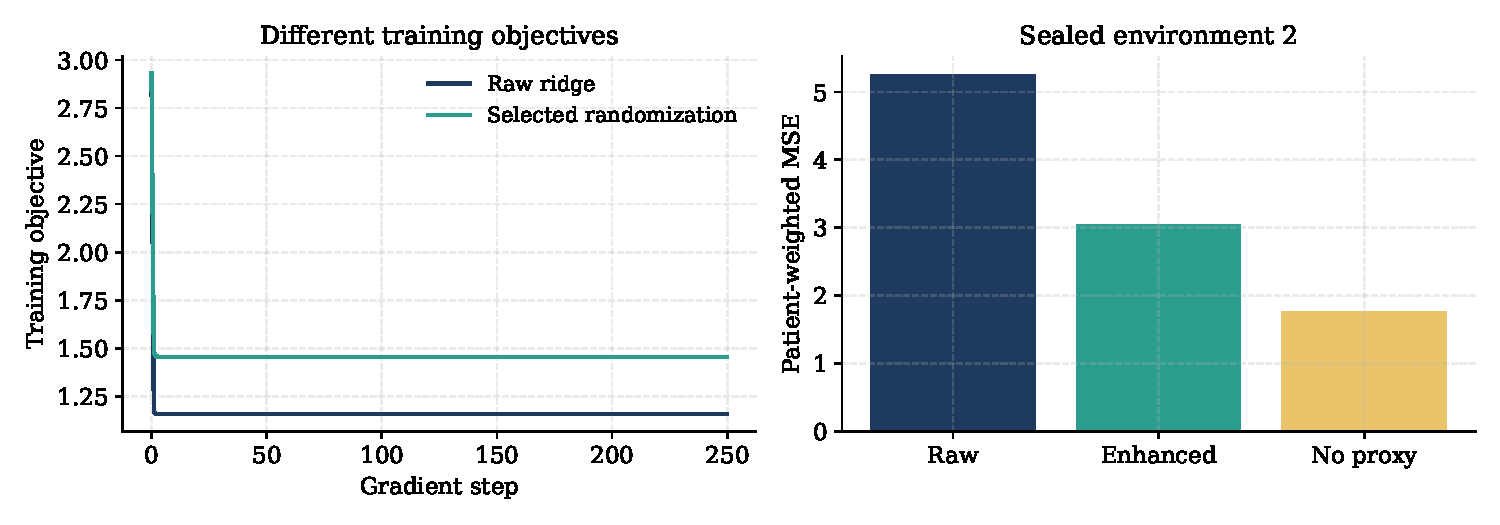
\includegraphics[width=\textwidth]{figs/causal_training.pdf}
\caption{Deterministic mini-project output for seed 0. Left: training objectives,
which differ after randomization and should not be compared as the same loss.
Right: all models evaluated with the same patient-weighted test MSE in environment 2.}
\end{figure}

\section{The informative ablation is better}
Removing the proxy entirely gives a lower test error than the selected enhancement.
The selected model retains a small amount of proxy dependence because that helps on
source validation. Environment 2 reverses the relationship. The source criterion does
not reveal which unobserved target shift will occur.

This result should not be hidden by rerunning selection on the test environment.
The predefined ablation explains where the remaining failure arises. It does not supply
an independent patient study and does not establish that removing a real biological
variable would improve prediction or effect identification.

\section{Variation across synthetic runs}
An independently rerun five-seed comparison with unchanged default settings yields
the following means and sample standard deviations over seeds $0,1,2,3,4$:
\begin{center}
\begin{tabular}{lrr}
\toprule
Quantity & Mean & Sample SD\\
\midrule
Naive ATE & 2.2069 & 0.0127\\
Adjusted ATE & 1.0006 & 0.0032\\
Raw test MSE & 5.2523 & 0.7800\\
Selected enhancement test MSE & 2.2166 & 0.7492\\
No-proxy ablation test MSE & 1.7898 & 0.2008\\
Training-mean test MSE & 3.3271 & 0.2624\\
\bottomrule
\end{tabular}
\end{center}
Seeds 0 and 1 select $p=0.5$; seeds 2, 3, and 4 select $p=1$.
These standard deviations summarize simulator/run variability, not a patient-population
confidence interval. More seeds would refine that numerical summary without validating
the missing causal assumptions.

\section{Uncertainty and a changed mechanism}
The report also includes a percentile bootstrap interval for selected-model test MSE.
It resamples whole patients' mean squared errors after model selection. This describes
sampling variation conditional on the fitted model and a representative independent
patient sample. It does not include model-training variability, graph selection,
measurement-model error, or violation of transport assumptions.

Try \texttt{--target-shift 1}. The test target changes from coefficient 1.5 on $Z$
to 2.5. A predictor omitting the nuisance still uses a source-fitted coefficient,
so stable features alone cannot repair this target-mechanism change. Report the
same predefined models; avoid adapting the procedure after seeing test labels.

\begin{pitfall}
An observed MSE improvement is evidence about prediction on the evaluated fixture.
It does not establish the true biological graph, a new target's effect, or a clinical
benefit. A seed SD and a conditional patient bootstrap answer different uncertainty questions.
\end{pitfall}

\chapter{Safety angle}
\begin{safetyangle}
\section{Match the claim to the evidence}
The most consequential failure is to turn a useful computational hypothesis into a
verified intervention claim without the needed identification and validation. Explicitly
name the estimand, assumptions, context, and supporting data. A graph endpoint that remains
uncertain should stay uncertain in a target-prioritization explanation.

For observational treatment data, confounding, selection, and measurement can each
prevent the desired causal interpretation. The toy adjusted estimator assumes the
relevant confounder is measured; it cannot repair a hidden common cause or a poorly
specified treatment version. Hern\'an and Robins' \emph{What If} provides the appropriate
effect-identification background.

\section{Enhancement can preserve a task and harm another}
An enhancement model can improve reconstruction, classification, or segmentation while
altering conditional independences. Causal discovery cares about those dependencies.
Negative controls should therefore be specific to the intended structure-learning claim,
not merely to how smooth a heat map looks. The imputation study by Andrews and Hemberg
motivates separate assessment of false signals.

Retain raw measurements and transformation provenance. Report unchanged-data baselines,
ablations, and held-out contexts. For biological hypotheses, follow-up perturbations,
appropriate controls, timing, and relevant cell states supply a different kind of evidence
from a new random split of the same donors.

\section{Selection and patient grouping}
Split before fitting preprocessing, enhancement, or feature selection. Group by the unit
that can share hidden information: patient, donor, specimen, or study as appropriate.
An independent donor test can still fail to test transport if chemistry or study effects
are duplicated on both sides. Environment and patient holdouts answer complementary questions.

Resampling individual cells for a patient-level interval can produce artificially narrow
uncertainty by counting correlated observations as independent. The project's patient
bootstrap is a limited remedy for its stated fixed-model metric, not a universal design.
\end{safetyangle}

\section{An evidence ladder for a proposed target}
A practical hypothesis record can say: a candidate edge is compatible with the data
and assumptions; a specified graph family leaves some alternatives; a target intervention
prediction follows from a selected model; a controlled perturbation tests part of that
prediction; additional contexts assess transport. These are cumulative claims with
different uncertainty, not interchangeable scores.

For example, an expression marker may predict an outcome because it is downstream of
the disease process. Reducing that marker's measured value does not necessarily change
the disease. A causal model should make this possibility explicit before suggesting
which experiment would distinguish the alternatives.

\section{A useful negative-control design}
One course extension is to independently permute two synthetic marker columns within
training patients, creating known absent cross-marker dependencies, then pass them through
an enhancement pipeline. If that pipeline induces strong shared structure, report it as
an artifact under this control. Keep its scope precise: the control diagnoses this
operation and fixture, not all possible real biological signals.

\begin{pitfall}
Passing the code's leakage tests establishes concrete programming contracts. It does
not establish that a real patient identifier is complete, that cohorts are representative,
or that an intervention model is biologically correct.
\end{pitfall}

\chapter{Matching application}
\begin{matching}
\section{Association and incremental value can rank differently}
Consider a synthetic lead router with capacity to contact two of three leads. A prediction
score estimates an observed association with an outcome; the causal objective is the
incremental outcome from contact compared with no contact. Existing customer intent
can raise both the chance of contact and the chance of success, confounding the observed
contact association.

The association scores are $(0.9,0.8,0.1)$ and the simulator's improvements are
$(-0.2,0.5,1.0)$. Ranking by association chooses leads 0 and 1. Its average improvement
is $(-0.2+0.5)/2=0.15$. Ranking by the known synthetic effects chooses leads 2 and 1,
giving $(1.0+0.5)/2=0.75$.

\texttt{exercise\_8\_matching\_priority\_value} computes this fixed-shortlist metric.
The potential improvements are supplied by the simulator. An ordinary historical log
contains only the outcome of the action actually taken, so the same calculation is not
identified without additional evidence and assumptions.
\end{matching}

\section{Transfer to candidate matching}
In recruitment, a model might predict who will be hired under the current process.
That is different from estimating the incremental value of an interview or training
intervention. An employer or job family can be an environment, while recorded recruitment
stage or recruiter behavior can create selection mechanisms. Repeated applications by
the same candidate require grouping analogous to repeated cells from one donor.

This translation explains why Week 11's support and Week 25's audit concerns still matter.
A new environment does not automatically provide a randomized treatment assignment,
and an enhanced candidate representation does not make an observational hiring label
an unbiased treatment effect.

\section{An objective must include its constraints}
Capacity, eligibility, and the meaning of the unit should be stated before reporting
value. A shortlist ranking metric does not evaluate unseen candidates. A model might
improve a global outcome while increasing error in a rare subgroup or a new job context.
The appropriate metric and constraints depend on the user's decision, rather than being
determined by whichever number the optimizer returns.

Use a concrete memo: ``In this simulator, with a budget of two and known potential
improvements, effect ranking achieves mean improvement 0.75.'' Do not expand it into
a claim that the ranker is fair, clinically effective, or validated for a real population.
\begin{pitfall}
Observed success, calibrated prediction, incremental treatment benefit, and exposure
fairness use different denominators and counterfactual questions. One good score does
not identify all four.
\end{pitfall}

\chapter{Exercises}
The workbook supplies full prompts, collapsible hints, learner scaffolds, and checks.
Its default path uses labeled reference implementations. A learner attempt intentionally
stops with \texttt{NotImplementedError} until completed; a reference run is not a graded submission.

\begin{enumerate}
\item \textbf{$\star$ Observed difference.} Compute the pooled treated-minus-untreated
mean in the 200-unit severity fixture. Predict its sign, then reconstruct its numerator
and denominator. State why the answer differs from the simulator's effect.
\begin{intuition}The treated and untreated severity mixtures differ.\end{intuition}

\item \textbf{$\star\star$ Standardization.} Derive the adjustment formula and implement
it for categorical strata. Reject a missing treatment cell. Repeat with a new target
mixture and explain whether equal stratum effects change the ATE.
\begin{intuition}Use one common population distribution for both potential-outcome means.\end{intuition}

\item \textbf{$\star\star$ Equivalent SCMs.} Calculate both covariance matrices for
the forward and reverse Gaussian models. Determine each mean under
$\operatorname{do}(X=1)$. Describe an experiment that could distinguish the directions
and a context assumption needed to interpret it.
\begin{intuition}Intervention replaces an assignment; it does not condition on a regression input.\end{intuition}

\item \textbf{$\star\star$ Patient split.} Hold out environment 2 and stratify the other
environments by patient. Check disjoint patient ID sets and allocation of every row.
Explain what to do if a donor appears across studies under different local IDs.
\begin{intuition}Globally unique identifiers are part of the data contract.\end{intuition}

\item \textbf{$\star\star$ Frozen imputation.} Fit observed-only means on training data,
preserve biological zeros, and transform held-out rows without fitting. Analyze an
all-missing column and an MNAR mechanism that violates the toy missingness premise.
\begin{intuition}A numerical fallback does not restore unobserved information.\end{intuition}

\item \textbf{$\star\star$ Residual diagnostic.} Compute mean and variance spread for
two environments with residuals $(-1,1)$ and $(-2,2)$. Explain the difference between
this description and a calibrated invariant-mechanism test.
\begin{intuition}Equal first moments do not imply equal distributions.\end{intuition}

\item \textbf{$\star\star$ Task-specific randomization.} Permute a seeded fraction of
one training nuisance column; preserve the source array and other columns. Show what
is preserved at $p=1$. Explain why the same transformation could invalidate a
structure-learning task.
\begin{intuition}Labels stay fixed only because this fixture's nuisance does not generate them.\end{intuition}

\item \textbf{$\star\star\star$ Matching and transfer.} Compare association ranking
with known-effect ranking under a capacity of two. Then run the prediction experiment
over seeds 0--4 and with a target-mechanism change. Write a memo separating prediction,
effect identification, graph ambiguity, and follow-up perturbation evidence.
\begin{intuition}Report the predefined no-proxy ablation even when it beats the selected enhancement.\end{intuition}
\end{enumerate}

\section{A memo that makes its assumptions reviewable}
Start with the population and intervention question. State which variables and mechanisms
are measured, which can change, and which are held stable. Give the patient grouping rule
and identify the data used for fitting, selection, and testing. Report the baseline,
enhancement, ablation, and uncertainty with the same metric. Finish by naming an unresolved
causal alternative and the evidence that could distinguish it.

The reference memo outline in the notebook is an interpretation aid, not an automated
causal assessment. Passing all fixture assertions leaves the central scientific task:
deciding whether the stated assumptions describe the real system.

\begin{pitfall}
Checking a reference solution against itself does not evaluate learner code. The
workbook selects either a learner function or a labeled reference function and then
checks that selected implementation against explicit fixture expectations.
\end{pitfall}

\chapter{Further reading}
\texttt{extended\_reading.pdf} annotates five public papers on multi-environment
discovery, invariant prediction, task-driven augmentation, imputation artifacts, and
noisy subspace learning. The book \emph{Causal Inference: What If} supplies the deeper
effect-estimation sequence. Read the source dossier to distinguish company descriptions,
peer-reviewed results, preprints, and course-created examples. None of these citations
extends an omitted algorithm's guarantee to this project.

\section{Source links}
\begin{enumerate}
\item Hern\'an and Robins (2020), \emph{Causal Inference: What If}.
\url{https://miguelhernan.org/whatifbook}.
\item Li, Jaber, and Bareinboim (2023), NeurIPS 36, multi-environment causal discovery.
\url{https://proceedings.neurips.cc/paper_files/paper/2023/hash/368cba57d00902c752eaa9e4770bbbbe-Abstract-Conference.html}.
\item Peters, B\"uhlmann, and Meinshausen (2016), invariant causal prediction,
\texttt{arXiv:1501.01332}. \url{https://arxiv.org/abs/1501.01332}.
\item Mooij, Magliacane, and Claassen (2020), JCI, JMLR 21(99).
\url{https://jmlr.org/papers/v21/17-123.html}.
\item Andrews and Hemberg (2018; revised 2019), imputation artifacts.
\url{https://f1000research.com/articles/7-1740}.
\end{enumerate}

\section{Questions for the discussion}
What constitutes an environment, and which mechanisms can change? What graph endpoints
remain unresolved? Which assumptions justify the virtual intervention? Which downstream
objective trains enhancement, and what negative controls detect manufactured dependencies?
Are all models and transformations evaluated on independent patients and contexts?
Which controlled perturbations test predictions in the relevant cell state?

\begin{pitfall}
A talk announcement does not disclose a reproducible method. The lesson does not
attribute its nuisance permutation, ICP diagnostic, or NumPy model to either speaker
or to Synlico's proprietary system.
\end{pitfall}
\paragraph{Sourced from.} The dated bibliography and provenance are in
\href{../research/causal_biology.md}{\texttt{research/causal\_biology.md}}.
Related support/audit background is in
\href{../research/bandits_matching_sota.md}{\texttt{research/bandits\_matching\_sota.md}}.
\end{document}
